% Options for packages loaded elsewhere
\PassOptionsToPackage{unicode}{hyperref}
\PassOptionsToPackage{hyphens}{url}
\PassOptionsToPackage{dvipsnames,svgnames,x11names}{xcolor}
%
\documentclass[
  letterpaper,
  DIV=11,
  numbers=noendperiod]{scrartcl}

\usepackage{amsmath,amssymb}
\usepackage{iftex}
\ifPDFTeX
  \usepackage[T1]{fontenc}
  \usepackage[utf8]{inputenc}
  \usepackage{textcomp} % provide euro and other symbols
\else % if luatex or xetex
  \usepackage{unicode-math}
  \defaultfontfeatures{Scale=MatchLowercase}
  \defaultfontfeatures[\rmfamily]{Ligatures=TeX,Scale=1}
\fi
\usepackage{lmodern}
\ifPDFTeX\else  
    % xetex/luatex font selection
\fi
% Use upquote if available, for straight quotes in verbatim environments
\IfFileExists{upquote.sty}{\usepackage{upquote}}{}
\IfFileExists{microtype.sty}{% use microtype if available
  \usepackage[]{microtype}
  \UseMicrotypeSet[protrusion]{basicmath} % disable protrusion for tt fonts
}{}
\makeatletter
\@ifundefined{KOMAClassName}{% if non-KOMA class
  \IfFileExists{parskip.sty}{%
    \usepackage{parskip}
  }{% else
    \setlength{\parindent}{0pt}
    \setlength{\parskip}{6pt plus 2pt minus 1pt}}
}{% if KOMA class
  \KOMAoptions{parskip=half}}
\makeatother
\usepackage{xcolor}
\usepackage{svg}
\usepackage{soul}
\setlength{\emergencystretch}{3em} % prevent overfull lines
\setcounter{secnumdepth}{5}
% Make \paragraph and \subparagraph free-standing
\ifx\paragraph\undefined\else
  \let\oldparagraph\paragraph
  \renewcommand{\paragraph}[1]{\oldparagraph{#1}\mbox{}}
\fi
\ifx\subparagraph\undefined\else
  \let\oldsubparagraph\subparagraph
  \renewcommand{\subparagraph}[1]{\oldsubparagraph{#1}\mbox{}}
\fi

\usepackage{color}
\usepackage{fancyvrb}
\newcommand{\VerbBar}{|}
\newcommand{\VERB}{\Verb[commandchars=\\\{\}]}
\DefineVerbatimEnvironment{Highlighting}{Verbatim}{commandchars=\\\{\}}
% Add ',fontsize=\small' for more characters per line
\usepackage{framed}
\definecolor{shadecolor}{RGB}{241,243,245}
\newenvironment{Shaded}{\begin{snugshade}}{\end{snugshade}}
\newcommand{\AlertTok}[1]{\textcolor[rgb]{0.68,0.00,0.00}{#1}}
\newcommand{\AnnotationTok}[1]{\textcolor[rgb]{0.37,0.37,0.37}{#1}}
\newcommand{\AttributeTok}[1]{\textcolor[rgb]{0.40,0.45,0.13}{#1}}
\newcommand{\BaseNTok}[1]{\textcolor[rgb]{0.68,0.00,0.00}{#1}}
\newcommand{\BuiltInTok}[1]{\textcolor[rgb]{0.00,0.23,0.31}{#1}}
\newcommand{\CharTok}[1]{\textcolor[rgb]{0.13,0.47,0.30}{#1}}
\newcommand{\CommentTok}[1]{\textcolor[rgb]{0.37,0.37,0.37}{#1}}
\newcommand{\CommentVarTok}[1]{\textcolor[rgb]{0.37,0.37,0.37}{\textit{#1}}}
\newcommand{\ConstantTok}[1]{\textcolor[rgb]{0.56,0.35,0.01}{#1}}
\newcommand{\ControlFlowTok}[1]{\textcolor[rgb]{0.00,0.23,0.31}{#1}}
\newcommand{\DataTypeTok}[1]{\textcolor[rgb]{0.68,0.00,0.00}{#1}}
\newcommand{\DecValTok}[1]{\textcolor[rgb]{0.68,0.00,0.00}{#1}}
\newcommand{\DocumentationTok}[1]{\textcolor[rgb]{0.37,0.37,0.37}{\textit{#1}}}
\newcommand{\ErrorTok}[1]{\textcolor[rgb]{0.68,0.00,0.00}{#1}}
\newcommand{\ExtensionTok}[1]{\textcolor[rgb]{0.00,0.23,0.31}{#1}}
\newcommand{\FloatTok}[1]{\textcolor[rgb]{0.68,0.00,0.00}{#1}}
\newcommand{\FunctionTok}[1]{\textcolor[rgb]{0.28,0.35,0.67}{#1}}
\newcommand{\ImportTok}[1]{\textcolor[rgb]{0.00,0.46,0.62}{#1}}
\newcommand{\InformationTok}[1]{\textcolor[rgb]{0.37,0.37,0.37}{#1}}
\newcommand{\KeywordTok}[1]{\textcolor[rgb]{0.00,0.23,0.31}{#1}}
\newcommand{\NormalTok}[1]{\textcolor[rgb]{0.00,0.23,0.31}{#1}}
\newcommand{\OperatorTok}[1]{\textcolor[rgb]{0.37,0.37,0.37}{#1}}
\newcommand{\OtherTok}[1]{\textcolor[rgb]{0.00,0.23,0.31}{#1}}
\newcommand{\PreprocessorTok}[1]{\textcolor[rgb]{0.68,0.00,0.00}{#1}}
\newcommand{\RegionMarkerTok}[1]{\textcolor[rgb]{0.00,0.23,0.31}{#1}}
\newcommand{\SpecialCharTok}[1]{\textcolor[rgb]{0.37,0.37,0.37}{#1}}
\newcommand{\SpecialStringTok}[1]{\textcolor[rgb]{0.13,0.47,0.30}{#1}}
\newcommand{\StringTok}[1]{\textcolor[rgb]{0.13,0.47,0.30}{#1}}
\newcommand{\VariableTok}[1]{\textcolor[rgb]{0.07,0.07,0.07}{#1}}
\newcommand{\VerbatimStringTok}[1]{\textcolor[rgb]{0.13,0.47,0.30}{#1}}
\newcommand{\WarningTok}[1]{\textcolor[rgb]{0.37,0.37,0.37}{\textit{#1}}}

\providecommand{\tightlist}{%
  \setlength{\itemsep}{0pt}\setlength{\parskip}{0pt}}\usepackage{longtable,booktabs,array}
\usepackage{calc} % for calculating minipage widths
% Correct order of tables after \paragraph or \subparagraph
\usepackage{etoolbox}
\makeatletter
\patchcmd\longtable{\par}{\if@noskipsec\mbox{}\fi\par}{}{}
\makeatother
% Allow footnotes in longtable head/foot
\IfFileExists{footnotehyper.sty}{\usepackage{footnotehyper}}{\usepackage{footnote}}
\makesavenoteenv{longtable}
\usepackage{graphicx}
\makeatletter
\def\maxwidth{\ifdim\Gin@nat@width>\linewidth\linewidth\else\Gin@nat@width\fi}
\def\maxheight{\ifdim\Gin@nat@height>\textheight\textheight\else\Gin@nat@height\fi}
\makeatother
% Scale images if necessary, so that they will not overflow the page
% margins by default, and it is still possible to overwrite the defaults
% using explicit options in \includegraphics[width, height, ...]{}
\setkeys{Gin}{width=\maxwidth,height=\maxheight,keepaspectratio}
% Set default figure placement to htbp
\makeatletter
\def\fps@figure{htbp}
\makeatother
\newlength{\cslhangindent}
\setlength{\cslhangindent}{1.5em}
\newlength{\csllabelwidth}
\setlength{\csllabelwidth}{3em}
\newlength{\cslentryspacingunit} % times entry-spacing
\setlength{\cslentryspacingunit}{\parskip}
\newenvironment{CSLReferences}[2] % #1 hanging-ident, #2 entry spacing
 {% don't indent paragraphs
  \setlength{\parindent}{0pt}
  % turn on hanging indent if param 1 is 1
  \ifodd #1
  \let\oldpar\par
  \def\par{\hangindent=\cslhangindent\oldpar}
  \fi
  % set entry spacing
  \setlength{\parskip}{#2\cslentryspacingunit}
 }%
 {}
\usepackage{calc}
\newcommand{\CSLBlock}[1]{#1\hfill\break}
\newcommand{\CSLLeftMargin}[1]{\parbox[t]{\csllabelwidth}{#1}}
\newcommand{\CSLRightInline}[1]{\parbox[t]{\linewidth - \csllabelwidth}{#1}\break}
\newcommand{\CSLIndent}[1]{\hspace{\cslhangindent}#1}

\usepackage{booktabs}
\usepackage{longtable}
\usepackage{array}
\usepackage{multirow}
\usepackage{wrapfig}
\usepackage{float}
\usepackage{colortbl}
\usepackage{pdflscape}
\usepackage{tabu}
\usepackage{threeparttable}
\usepackage{threeparttablex}
\usepackage[normalem]{ulem}
\usepackage{makecell}
\usepackage{xcolor}
\KOMAoption{captions}{tableheading}
\makeatletter
\makeatother
\makeatletter
\makeatother
\makeatletter
\@ifpackageloaded{caption}{}{\usepackage{caption}}
\AtBeginDocument{%
\ifdefined\contentsname
  \renewcommand*\contentsname{Table of contents}
\else
  \newcommand\contentsname{Table of contents}
\fi
\ifdefined\listfigurename
  \renewcommand*\listfigurename{List of Figures}
\else
  \newcommand\listfigurename{List of Figures}
\fi
\ifdefined\listtablename
  \renewcommand*\listtablename{List of Tables}
\else
  \newcommand\listtablename{List of Tables}
\fi
\ifdefined\figurename
  \renewcommand*\figurename{Figure}
\else
  \newcommand\figurename{Figure}
\fi
\ifdefined\tablename
  \renewcommand*\tablename{Table}
\else
  \newcommand\tablename{Table}
\fi
}
\@ifpackageloaded{float}{}{\usepackage{float}}
\floatstyle{ruled}
\@ifundefined{c@chapter}{\newfloat{codelisting}{h}{lop}}{\newfloat{codelisting}{h}{lop}[chapter]}
\floatname{codelisting}{Listing}
\newcommand*\listoflistings{\listof{codelisting}{List of Listings}}
\makeatother
\makeatletter
\@ifpackageloaded{caption}{}{\usepackage{caption}}
\@ifpackageloaded{subcaption}{}{\usepackage{subcaption}}
\makeatother
\makeatletter
\@ifpackageloaded{tcolorbox}{}{\usepackage[skins,breakable]{tcolorbox}}
\makeatother
\makeatletter
\@ifundefined{shadecolor}{\definecolor{shadecolor}{rgb}{.97, .97, .97}}
\makeatother
\makeatletter
\makeatother
\makeatletter
\makeatother
\ifLuaTeX
  \usepackage{selnolig}  % disable illegal ligatures
\fi
\IfFileExists{bookmark.sty}{\usepackage{bookmark}}{\usepackage{hyperref}}
\IfFileExists{xurl.sty}{\usepackage{xurl}}{} % add URL line breaks if available
\urlstyle{same} % disable monospaced font for URLs
\hypersetup{
  pdftitle={Amazing Document},
  pdfauthor={Filippo Gambarota},
  colorlinks=true,
  linkcolor={blue},
  filecolor={Maroon},
  citecolor={Blue},
  urlcolor={Blue},
  pdfcreator={LaTeX via pandoc}}

\title{Amazing Document}
\usepackage{etoolbox}
\makeatletter
\providecommand{\subtitle}[1]{% add subtitle to \maketitle
  \apptocmd{\@title}{\par {\large #1 \par}}{}{}
}
\makeatother
\subtitle{Amazing Location}
\author{Filippo Gambarota}
\date{2023-09-05}

\begin{document}
\maketitle
\ifdefined\Shaded\renewenvironment{Shaded}{\begin{tcolorbox}[sharp corners, borderline west={3pt}{0pt}{shadecolor}, breakable, frame hidden, interior hidden, enhanced, boxrule=0pt]}{\end{tcolorbox}}\fi

\renewcommand*\contentsname{Table of contents}
{
\hypersetup{linkcolor=}
\setcounter{tocdepth}{3}
\tableofcontents
}
\hypertarget{quarto}{%
\section{Quarto}\label{quarto}}

\hypertarget{general-markup}{%
\subsection{General Markup}\label{general-markup}}

You can write standard markdown code. Using \textbf{bold}, \emph{italic}
or \st{underlined} text. You can include an external figure and also
using cross reference with \texttt{@fig-quarto} that produce
Figure~\ref{fig-quarto}

\begin{figure}

{\centering \includesvg{pdf-example_files/mediabag/quarto.svg}

}

\caption{\label{fig-quarto}My beautiful caption}

\end{figure}

\hypertarget{math}{%
\subsection{Math}\label{math}}

You can write math using Latex code:

\begin{Shaded}
\begin{Highlighting}[]
\SpecialStringTok{$$}
\SpecialStringTok{y = }\SpecialCharTok{\textbackslash{}beta}\SpecialStringTok{\_0 + }\SpecialCharTok{\textbackslash{}beta}\SpecialStringTok{\_1 + }\SpecialCharTok{\textbackslash{}epsilon}
\SpecialStringTok{$$}
\end{Highlighting}
\end{Shaded}

\[
y = \beta_0 + \beta_1 + \epsilon
\]

And also inline math using \texttt{\$\textbackslash{}alpha\$} that
produce \(\alpha\)

\hypertarget{sec-citations}{%
\subsection{Citations}\label{sec-citations}}

You can cite references from a \texttt{.bib} file using the syntax
\texttt{{[}@Chen2021-jb{]}} that produce (Chen et al. 2021). We can also
cite multiple authors \texttt{{[}@Morey2011-zc;\ @Lakens2018-ri{]}}
(Morey and Rouder 2011; Lakens, Scheel, and Isager 2018) or suppress the
author name \texttt{{[}-@Valentine2011-yq{]}} (2011).

A reference section will be automatically created at the end of the
document (see Section~\ref{sec-refs}).

\hypertarget{code-chunks}{%
\subsection{Code chunks}\label{code-chunks}}

The real beauty is including code chunks. Let's do some computations.
This is a code chunk as written in the source file.

\begin{Shaded}
\begin{Highlighting}[]
\NormalTok{\textasciigrave{}\textasciigrave{}\textasciigrave{}\{r\}}
\NormalTok{dat \textless{}{-} iris}
\NormalTok{summary(iris)}
\NormalTok{\textasciigrave{}\textasciigrave{}\textasciigrave{}}
\end{Highlighting}
\end{Shaded}

This is the result:

\begin{Shaded}
\begin{Highlighting}[]
\NormalTok{dat }\OtherTok{\textless{}{-}}\NormalTok{ iris}
\FunctionTok{summary}\NormalTok{(iris)}
\end{Highlighting}
\end{Shaded}

\begin{verbatim}
  Sepal.Length    Sepal.Width     Petal.Length    Petal.Width   
 Min.   :4.300   Min.   :2.000   Min.   :1.000   Min.   :0.100  
 1st Qu.:5.100   1st Qu.:2.800   1st Qu.:1.600   1st Qu.:0.300  
 Median :5.800   Median :3.000   Median :4.350   Median :1.300  
 Mean   :5.843   Mean   :3.057   Mean   :3.758   Mean   :1.199  
 3rd Qu.:6.400   3rd Qu.:3.300   3rd Qu.:5.100   3rd Qu.:1.800  
 Max.   :7.900   Max.   :4.400   Max.   :6.900   Max.   :2.500  
       Species  
 setosa    :50  
 versicolor:50  
 virginica :50  
                
                
                
\end{verbatim}

\hypertarget{code-chunks---plots}{%
\subsection{Code chunks - Plots}\label{code-chunks---plots}}

\begin{Shaded}
\begin{Highlighting}[]
\NormalTok{\textasciigrave{}\textasciigrave{}\textasciigrave{}\{r\}}
\NormalTok{library(ggplot2)}
\NormalTok{dat |\textgreater{}}
\NormalTok{    ggplot(aes(x = Sepal.Length, y = Petal.Width, color = Species)) +}
\NormalTok{    geom\_point() +}
\NormalTok{    geom\_smooth(method = "lm", se = FALSE) +}
\NormalTok{    theme\_minimal(20)}
\NormalTok{\textasciigrave{}\textasciigrave{}\textasciigrave{}}
\end{Highlighting}
\end{Shaded}

\begin{verbatim}
`geom_smooth()` using formula = 'y ~ x'
\end{verbatim}

\begin{figure}

{\centering 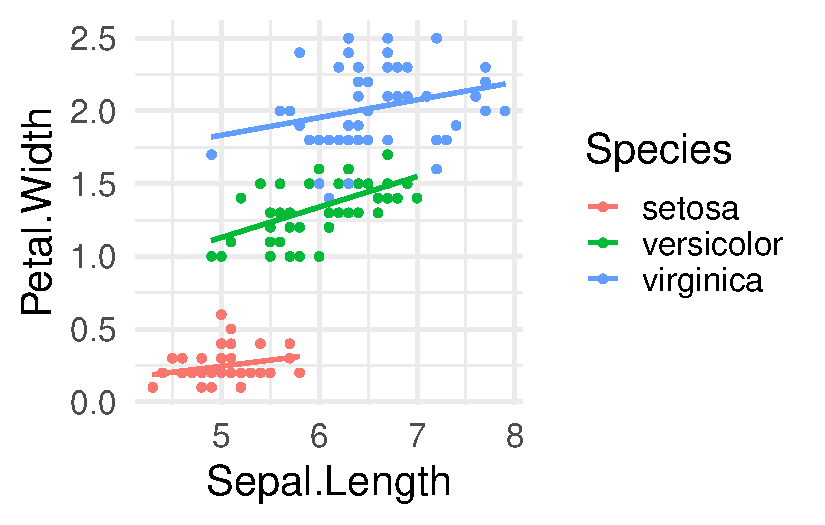
\includegraphics{pdf-example_files/figure-pdf/unnamed-chunk-4-1.pdf}

}

\end{figure}

\hypertarget{code-chunks---tables}{%
\subsection{Code chunks - Tables}\label{code-chunks---tables}}

You can also create already formatted tables with the statistics. Let's
fit a simple linear model:

\begin{Shaded}
\begin{Highlighting}[]
\NormalTok{fit }\OtherTok{\textless{}{-}} \FunctionTok{lm}\NormalTok{(Petal.Width }\SpecialCharTok{\textasciitilde{}}\NormalTok{ Sepal.Length }\SpecialCharTok{*}\NormalTok{ Species, }\AttributeTok{data =}\NormalTok{ dat)}
\FunctionTok{summary}\NormalTok{(fit)}
\end{Highlighting}
\end{Shaded}

\begin{verbatim}

Call:
lm(formula = Petal.Width ~ Sepal.Length * Species, data = dat)

Residuals:
     Min       1Q   Median       3Q      Max 
-0.56675 -0.10596 -0.02419  0.09624  0.50897 

Coefficients:
                               Estimate Std. Error t value Pr(>|t|)   
(Intercept)                    -0.17022    0.38833  -0.438  0.66180   
Sepal.Length                    0.08314    0.07739   1.074  0.28444   
Speciesversicolor               0.25348    0.49994   0.507  0.61292   
Speciesvirginica                1.39633    0.48104   2.903  0.00428 **
Sepal.Length:Speciesversicolor  0.12621    0.09371   1.347  0.18014   
Sepal.Length:Speciesvirginica   0.03827    0.08848   0.433  0.66599   
---
Signif. codes:  0 '***' 0.001 '**' 0.01 '*' 0.05 '.' 0.1 ' ' 1

Residual standard error: 0.1909 on 144 degrees of freedom
Multiple R-squared:  0.9394,    Adjusted R-squared:  0.9372 
F-statistic: 446.1 on 5 and 144 DF,  p-value: < 2.2e-16
\end{verbatim}

\hypertarget{code-chunks---tables-1}{%
\subsection{Code chunks - Tables}\label{code-chunks---tables-1}}

Let's produce the table with the \texttt{broom} and \texttt{kableExtra}
packages:

\begin{Shaded}
\begin{Highlighting}[]
\FunctionTok{library}\NormalTok{(kableExtra)}
\FunctionTok{library}\NormalTok{(broom)}

\NormalTok{fit }\SpecialCharTok{|\textgreater{}} 
\NormalTok{    broom}\SpecialCharTok{::}\FunctionTok{tidy}\NormalTok{() }\SpecialCharTok{|\textgreater{}} 
    \FunctionTok{kable}\NormalTok{() }\SpecialCharTok{|\textgreater{}} 
    \FunctionTok{kable\_styling}\NormalTok{(}\AttributeTok{full\_width =} \ConstantTok{FALSE}\NormalTok{,}
                  \AttributeTok{font\_size =} \DecValTok{20}\NormalTok{)}
\end{Highlighting}
\end{Shaded}

\begin{table}
\caption{My caption}\tabularnewline

\centering\begingroup\fontsize{20}{22}\selectfont

\begin{tabular}{l|r|r|r|r}
\hline
term & estimate & std.error & statistic & p.value\\
\hline
(Intercept) & -0.1702211 & 0.3883348 & -0.4383359 & 0.6617997\\
\hline
Sepal.Length & 0.0831444 & 0.0773861 & 1.0744106 & 0.2844357\\
\hline
Speciesversicolor & 0.2534768 & 0.4999386 & 0.5070159 & 0.6129192\\
\hline
Speciesvirginica & 1.3963295 & 0.4810424 & 2.9027162 & 0.0042819\\
\hline
Sepal.Length:Speciesversicolor & 0.1262127 & 0.0937089 & 1.3468601 & 0.1801412\\
\hline
Sepal.Length:Speciesvirginica & 0.0382720 & 0.0884806 & 0.4325467 & 0.6659912\\
\hline
\end{tabular}
\endgroup{}
\end{table}

\hypertarget{inline-code-chunks}{%
\subsection{Inline code chunks}\label{inline-code-chunks}}

If you want to use R code within the text to report statistics you can
use the syntax \texttt{\textasciigrave{}r\ r\ code\textasciigrave{}}.
For example:

\begin{itemize}
\tightlist
\item
  the average \texttt{Sepal.Length} for the \texttt{Setosa} group is
  \texttt{\textasciigrave{}r\ mean(iris\$Sepal.Length{[}iris\$Species\ ==\ \textquotesingle{}setosa\textquotesingle{}{]})\textasciigrave{}}
\end{itemize}

Become

\begin{itemize}
\tightlist
\item
  the average \texttt{Sepal.Length} for the \texttt{Setosa} group is
  5.006
\end{itemize}

\hypertarget{sec-refs}{%
\subsection{References}\label{sec-refs}}

Go back to Section~\ref{sec-citations}

\hypertarget{refs}{}
\begin{CSLReferences}{1}{0}
\leavevmode\vadjust pre{\hypertarget{ref-Chen2021-jb}{}}%
Chen, Gang, Daniel S Pine, Melissa A Brotman, Ashley R Smith, Robert W
Cox, and Simone P Haller. 2021. {``Trial and Error: A Hierarchical
Modeling Approach to Test-Retest Reliability.''} \emph{NeuroImage} 245
(December): 118647.
\url{https://doi.org/10.1016/j.neuroimage.2021.118647}.

\leavevmode\vadjust pre{\hypertarget{ref-Lakens2018-ri}{}}%
Lakens, Daniël, Anne M Scheel, and Peder M Isager. 2018. {``Equivalence
Testing for Psychological Research: A Tutorial.''} \emph{Adv. Methods
Pract. Psychol. Sci.} 1 (2): 259--69.
\url{https://doi.org/10.1177/2515245918770963}.

\leavevmode\vadjust pre{\hypertarget{ref-Morey2011-zc}{}}%
Morey, Richard D, and Jeffrey N Rouder. 2011. {``Bayes Factor Approaches
for Testing Interval Null Hypotheses.''} \emph{Psychol. Methods} 16 (4):
406--19. \url{https://doi.org/10.1037/a0024377}.

\leavevmode\vadjust pre{\hypertarget{ref-Valentine2011-yq}{}}%
Valentine, Jeffrey C, Anthony Biglan, Robert F Boruch, Felipe González
Castro, Linda M Collins, Brian R Flay, Sheppard Kellam, Eve K Mościcki,
and Steven P Schinke. 2011. {``Replication in Prevention Science.''}
\emph{Prev. Sci.} 12 (2): 103--17.
\url{https://doi.org/10.1007/s11121-011-0217-6}.

\end{CSLReferences}



\end{document}
